\documentclass[xcolor=dvipsnames]{beamer}

\usepackage[english]{babel}
\usepackage[latin1]{inputenc}
\usepackage[T1]{fontenc}

% --- Graphics inclusion.
\usepackage{graphicx}
%\usepackage{float}
%\usepackage{subfigure}
%\usepackage[all]{xy}

% --- Listing inclusion.
% \usepackage{dsfont}
% \usepackage{listings}
% \lstset{numbers=left, numberstyle=\tiny, numbersep=5pt}
% \lstset{language=C}

% --- Verbatim file inclusion.
%\usepackage{verbatim} % include entire files verbatim, \verbatiminput{...}

% --- Indent verbatim environments
\makeatletter \def\verbatim@startline{\verbatim@line{\leavevmode\kern20pt\relax}} \makeatother

% --- Color names.
%\usepackage{color}
%\usepackage[usenames,dvipsnames]{xcolor}
%\usepackage[svgnames]{xcolor}
% Define user colors using the RGB model
%\definecolor{darkgrey}{rgb}{0.8,0.8,0.8}
%\definecolor{lightgrey}{rgb}{0.95,0.95,0.95}
\definecolor{highlight}{named}{NavyBlue}

% --- Table mashups.
%\usepackage{colortbl}
%\usepackage{tabularx}
%\usepackage{longtable}
%\renewcommand*\arraystretch{2.0}

% --- Clubs and widows.
\clubpenalty = 10000
\widowpenalty = 10000
\displaywidowpenalty = 10000

% --- Vector fonts.
%\usepackage{mathptmx}
%\usepackage[scaled=.90]{helvet}
%\usepackage{courier}
%\usepackage{times} % True Type for normal text
%\usepackage{mathptmx} % True Type for maths

% --- Misc.
%\usepackage{trfrac}   % frac-like lines that are no fractions.
%\usepackage{moreverb} % More fun with {verbatim}
%\usepackage{amsfonts} % mathbb{N} and similar symbols
\usepackage{amsmath}  % \overset
\usepackage{amssymb}  % \ltimes
%\usepackage{pxfonts}  % \lJoin etc.; TypeSystems
%\setcounter{secnumdepth}{3}
%\setcounter{tocdepth}{3}


% ----- BEAMER SPECIFIC -----


% --- Pretty much the usual beamer theme.
\usepackage{beamerthemeshadow}

% --- A title slide for every new section.
\AtBeginSection{
  \frame{
    \begin{block}{}
      \begin{Large}\color{highlight}\centerline{\insertsection}\end{Large}
    \end{block}
  }
}

% --- Remove the navigation bar from the bottom right.
\beamertemplatenavigationsymbolsempty

% --- Fade in upcoming bullet points.
\beamersetuncovermixins{\opaqueness<1>{25}}{\opaqueness<2->{15}}




\begin{document}
\title{Visigoth.}
\author{}
\date{10 January 2012}

\frame{\titlepage}
\frame{\frametitle{Outline}\tableofcontents}


\section{Introduction}

\subsection{Motivation}
\frame{\frametitle{Motivation}
There is a whole class of barely explored graphs!
\pause

\vspace{0.5cm}
\emph{Example:} Graphs in social networks:
\pause

\begin{itemize}
  \item Facebook
  \item Twitter
  \item identi.ca
\end{itemize}
}

% FIXME: Not entirely happy with the slide split here.
%        Maybe we can write some more or put the points together?

\subsection{Small World Networks}
\frame{\frametitle{Small World Networks}
\begin{block}{Small World Networks}
  \emph{SWNs} are are graphs that look like a natural web of friendships.
\end{block}
}

\subsection{Small World Networks}
\frame{\frametitle{The Maths}
SWNs have certain properties:

\begin{enumerate}
  \pause
  \item Low average path Length
  \[ L_G = \frac{1}{N(N-1)} \sum_{i, j} d(v_i, v_j) \]
  \pause
  \item High clustering coefficient
  \[ C_i = \frac{2E_i}{k_i(k_i-1)} \]
  \pause
  \item Scale-free degree distribution 
\[ P(k) \sim k^{-\gamma} \]

\end{enumerate}

}

\subsection{Why SWNs?}
\frame{\frametitle{Why SWNs?}
SWNs are interesting because they show how people interact.

So let's have a look at them!
}

\subsection{Visigoth}
\frame{\frametitle{Visigoth}
Visigoth can generate or retrieve SWN graphs.

\vspace{0.5cm}
The user can analyse them both visually as well as statistically.

% FIXME: Screenshot here
\vspace{0.8cm}

\begin{figure}[h]
  \centering
  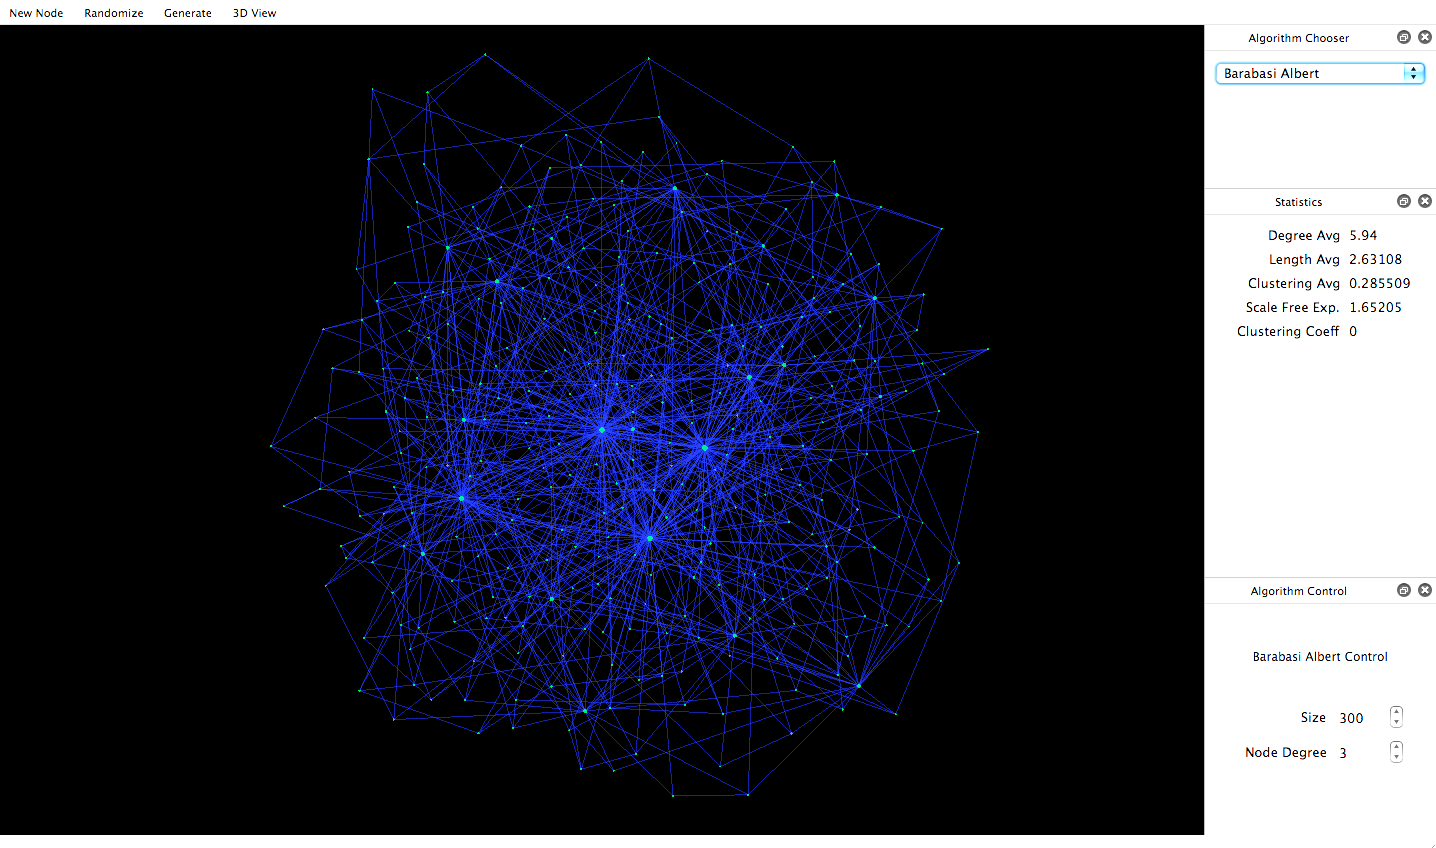
\includegraphics[height=30mm,width=60mm]{Fullscreen.png}
  \caption{Behold Visigoth}
  \label{fig:Visigoth}
\end{figure}

\vspace{0.8cm}
Really, this is the cutting edge in SWN science!
}



\section{Synthesis}

\subsection{SWN generation}

\frame{\frametitle{Generating SWNs, first attempt}
Let's grow a population. They will make friends with each other.\\
\pause
\hspace{0.5cm} $\to$ annoying (crying babies!)\\
\hspace{0.5cm} $\to$ expensive (feeding them!)\\
\hspace{0.5cm} $\to$ maybe a little too slow...
\pause

\vspace{0.5cm}
So what can we do?
}


\frame{\frametitle{Generating SWNs}
Okay, let's generate SWNs mathematically then.

That should be a lot more convenient!
\pause

\vspace{0.5cm}
Nowadays, we generate networks of \emph{thousands} of nodes within seconds.

\hspace{0.5cm} $\to$ 10,000 nodes within 3 sec
}

\frame{\frametitle{Algorithms}
We can generate graphs using several algorithms:

\vspace{0.5cm}
\begin{itemize}
  \item Erd\H{o}s-R\'{e}nyi
  \item Watts-Strogatz
  \item Barabasi-Albert
  \item Bipartite Model
  \item Preferential Attachment
\end{itemize}

\vspace{0.5cm}
... or just hack Facebook and get a huge social graph for free!
}


\subsection{Algorithms}

% FIXME: Don't forget to include example graphs.
%        Screenshots should be fine.
% Also, maybe we can combine 2 algos on 1 slide?
% We don't want to bore the audience.

\frame{\frametitle{Erd\H{o}s-R\'{e}nyi}
% FIXME: Text and screenshot here
\begin{itemize}
	\item Random Graph \dots
	\item \dots Therefore not SWN
	\item Completeness, Benchmark, Customer
\end{itemize}

\begin{figure}[h]
  \centering
  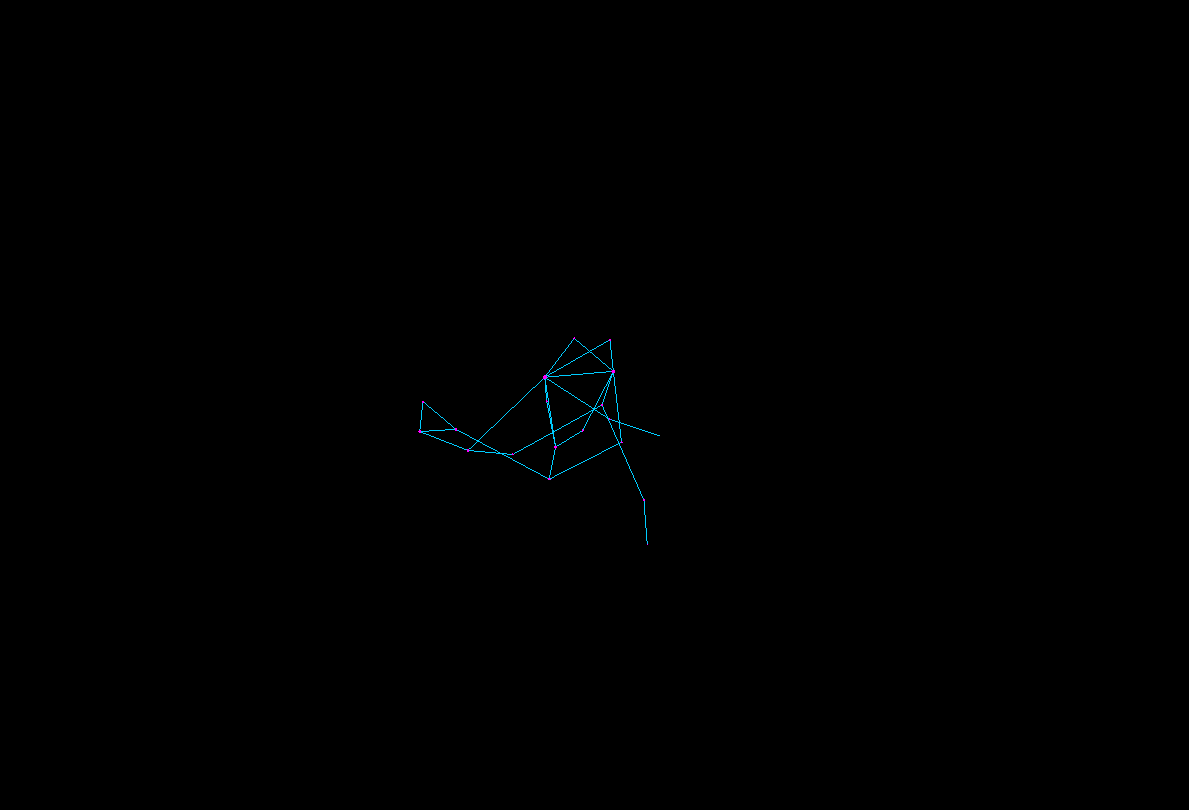
\includegraphics[height=30mm,width=60mm]{ErdosExport.png}
  \caption{Erd\H{o}s-R\'{e}nyi model generated by Visigoth}
  \label{fig:Erdos}
\end{figure}

}


\frame{\frametitle{Watts-Strogatz}
% FIXME: Text and screenshot here

\begin{itemize}
	\item Construct Ring Lattice
	\item Reconnect Random Edges
	\item Random Graph with SWN properties
	\item Certain SWN proerties i.e. High Clustering, Low Average Path
\end{itemize}

\begin{figure}[h]
  \centering
  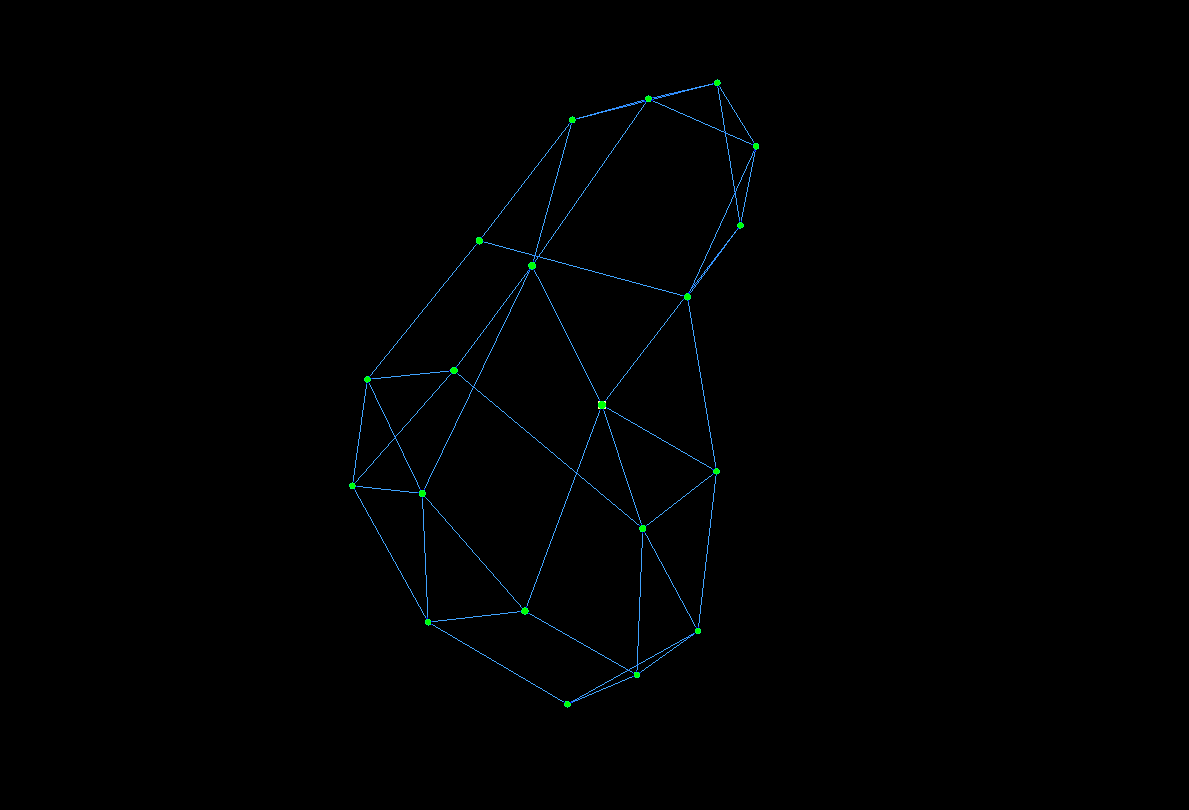
\includegraphics[height=30mm,width=60mm]{WattsExport.png}
  \caption{Watts-Strogatz model generated by Visigoth}
  \label{fig:Watts}
\end{figure}

}

\frame{\frametitle{Barabasi-Albert}
% FIXME: Text and screenshot here

\begin{itemize}
	\item Attach Nodes via Preferential Attachment
	\item SWN properties
	\item Scale-free Exponent, Low Average Path,
			Emperically Higher Clustering
\end{itemize}

\begin{figure}[h]
  \centering
  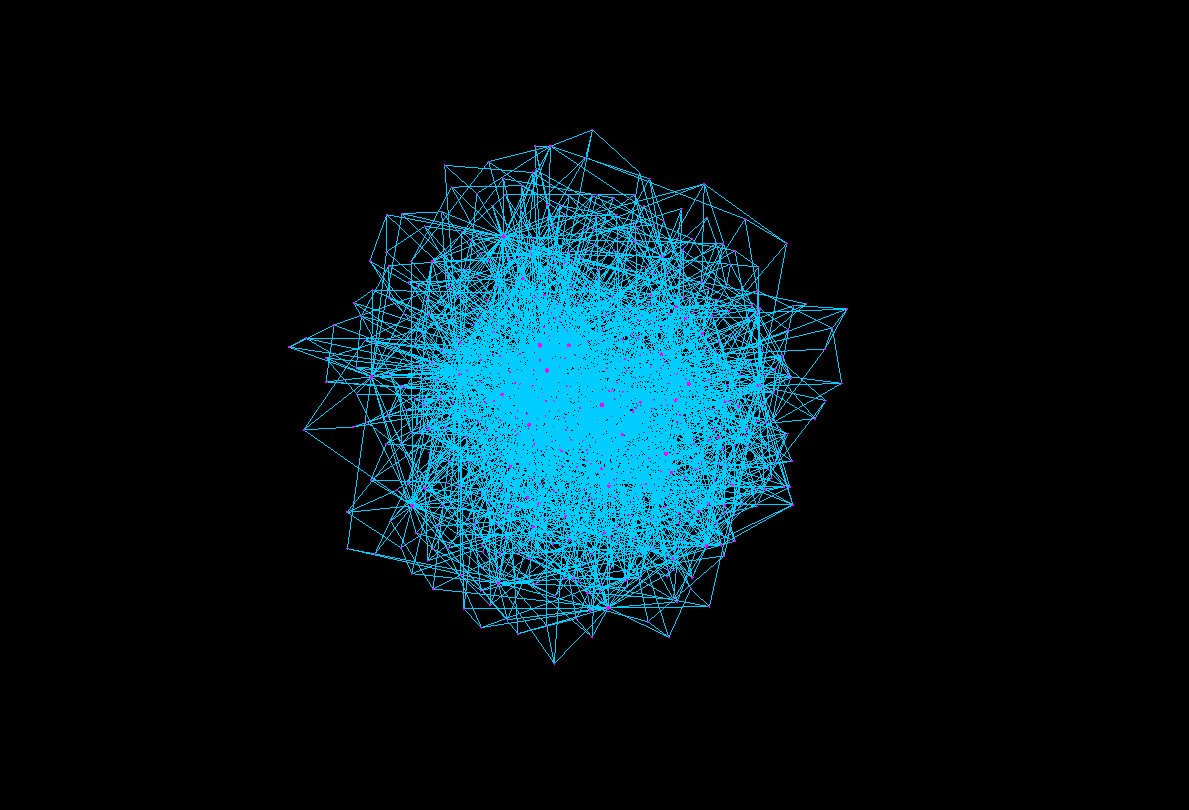
\includegraphics[height=30mm,width=60mm]{BarabasiExport.png}
  \caption{Barabasi-Albert model generated by Visigoth}
  \label{fig:Barabasi}
\end{figure}
}

\frame{\frametitle{Bipartite Model}
% FIXME: Text and screenshot here

\begin{itemize}
	\item Generate a Bipartite Graph
	\item Connect Nodes
	\item Collapse Graph
	\item Scale-free Exponent, Low Average Path,
			Emperically Higher Clustering
\end{itemize}

\begin{figure}[h]
  \centering
  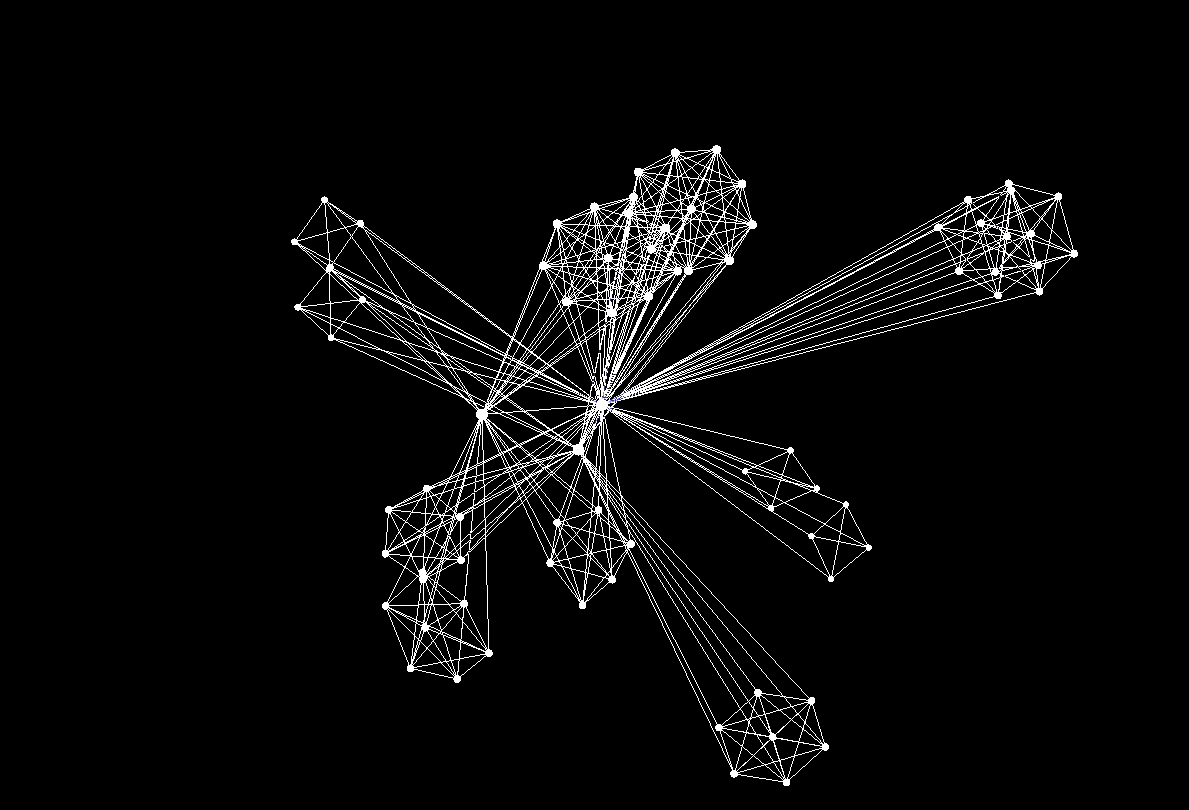
\includegraphics[height=25mm,width=60mm]{BipartiteExport.png}
  \caption{Biparite model generated by Visigoth}
  \label{fig:Bipartite}
\end{figure}
}

\frame{\frametitle{Preferential Attachment with Clustering}
% FIXME: Text and screenshot here

\begin{itemize}
	\item Attach Nodes via Preferential Attachment \dots
	\item \dots and Clustering
	\item SWN properties
	\item Scale-free Exponent, Low Average Path,
			Emperically Higher Clustering
\end{itemize}

\begin{figure}[h]
  \centering
  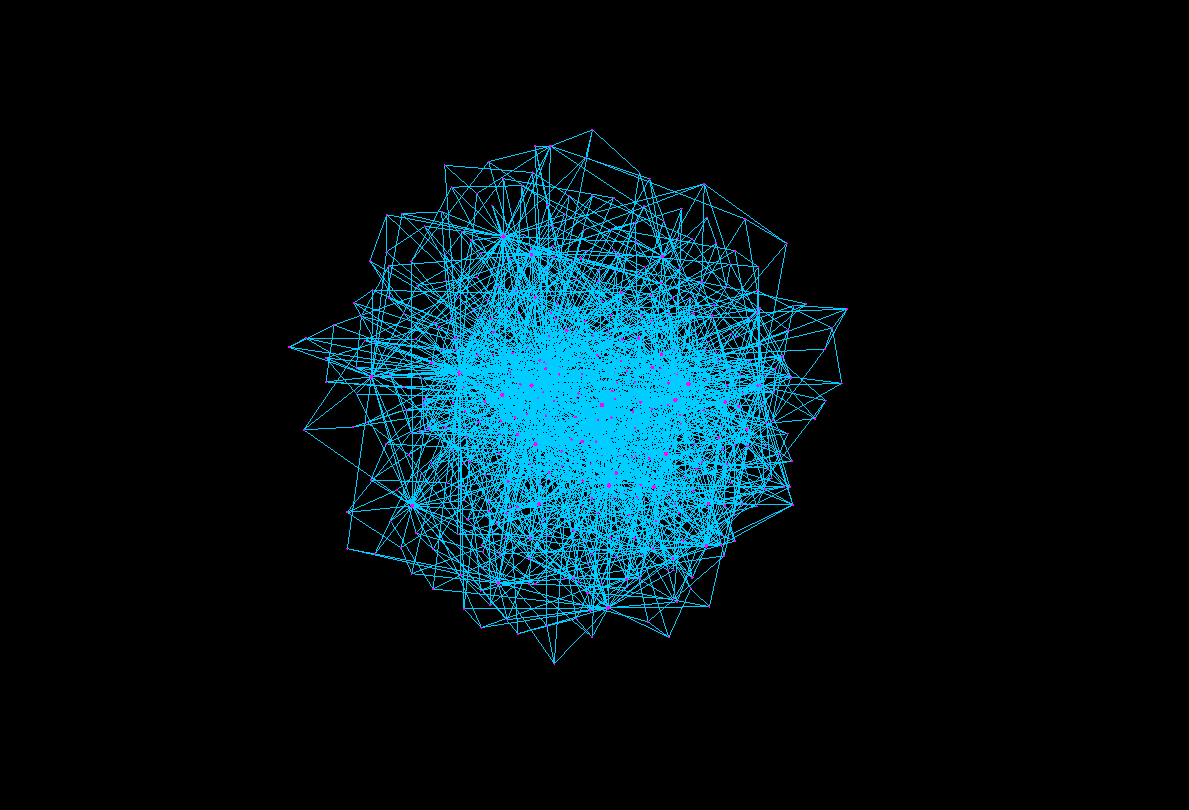
\includegraphics[height=25mm,width=60mm]{ClusteringExport.png}
  \caption{Preferential Attachment with Clustering model generated by Visigoth}
  \label{fig:Clustering}
\end{figure}
}

\frame{\frametitle{Real social networks}
% FIXME: Text and screenshot here
(text and screenshot here)
}

\subsection{Demo}
\frame{\frametitle{Demo}
It's demo time!
}



\section{Analysis}

\subsection{Statistics}
\frame{\frametitle{Statistical analysis}

\begin{itemize}
  \pause
  \item Average Path Length
  \pause
  \item Average Degree
  \pause
  \item Clustering Coefficient
  \pause
  \item Average Clustering Coefficient
  \pause
  \item Scale Free Exponent
  \pause 
  \item All in Real Time!

\end{itemize}
}

\subsection{Visuals}
\frame{\frametitle{Visual analysis}
Visigoth is a lot of fun for mouse addicts as well.

\vspace{0.5cm}
We can...

\begin{itemize}
  \pause
  \item Pan left/right/up/down
  \pause
  \item Zoom in/out.
  \pause
  \item And do it all in 3D!
\end{itemize}
}

\subsection{Visuals}
\frame{\frametitle{3D}
How we make the 3rd dimension reality....in Visigoth

\vspace{0.5cm}

\begin{itemize}
  \pause
  \item Open GL
\end{itemize}
}

% FIXME: Maybe add a slide about extra functionality, e.g. PNG export?

\subsection{Demo}
\frame{\frametitle{Demo}
It's demo time!
}

\subsection{Graph Customisation}
\frame{\frametitle{Graph Customisation}
If you think you can fit colors better than we do...

\pause
\vspace{0.5cm}
Visigoth lets you unleash the Picasso hidden inside yourself!
\pause
...by...

\begin{itemize}
\pause
\item Change the nodes and edges color
\pause
\item Change background color
\pause
\item Highlight selected nodes and their direct connections
\end{itemize}
}

\subsection{Demo}
\frame{\frametitle{Demo}
It's demo time!
}

\section{Engineering}

% FIXME: Teamwork, Tools (git), Methods (xP, agile, iterative, yadayada)


\section{Conclusion}







%% BEAMER EXAMPLES


\section{Example section 1}

\subsection{Subsec 1}

\frame{\frametitle{Slide Title. Pauses, bullet points}
Some text.
\pause

Some more text.
\pause

\begin{itemize}
  \item Bulletpoint 1.
  \pause
  \item Item 2 after a pause.
\end{itemize}
}


\subsection{Subsec 2}

\frame{\frametitle{Plain text}
Text....

\vspace{0.3cm}
More text....
}

\frame{\frametitle{Tables}
A table describing a Makefile
\vspace{0.5cm}

\begin{tabular}{ll}
  \texttt{make} & Compile\\
  \texttt{make run} & Run\\
  \texttt{make test} & Fail\\
  \texttt{make clean} & Clean up for distribution and inspection
\end{tabular}
}


\subsection{Huge tables}

\frame{\frametitle{Lotsa text}
This is a pretty full slide.
\vspace{0.5cm}

\begin{tabular}{ll}
  \texttt{Homer} & Family dad\\
  \texttt{Marge} & Family mom\\
  \\
  \texttt{Bart} & Son\\
  \texttt{Lisa} & Daughter\\
  \texttt{Maggie} & Teh baby\\
  \\
  \texttt{dog} & Not a cat.\\
  \texttt{cat} & Not a dog.\\
\end{tabular}

\vspace{0.3cm}
\begin{exampleblock}{How to seem surprised}
  \texttt{D'oh !}
\end{exampleblock}
}




\section{More examples}

\frame{\frametitle{No subsection}
This slide is outside the normal subsectioning.
\pause

\vspace{0.5cm}
This can be used for section introductions.
}


\subsection{Going wild}

\frame{\frametitle{Mixing pauses and spaces}
Cat drank\\
\pause
\hspace{0.5cm} $\to$ Alice found.
\pause

\vspace{0.5cm}
Dog ate\\
\pause
\hspace{0.5cm} $\to$ Alice found something else.
\pause

\vspace{0.5cm}
So what's the point, anyway?
}


\subsection{Tables, pauses, spaces, (non-)linebreaks}

\frame{\frametitle{SD card: Development}
Pause before a table. NOT in the table!
Also, some vspace.
\pause

\vspace{0.5cm}
But no linebreak after this line and before the table:
\begin{tabular}{rl}
  123 & not 321\\
  456 & 789
\end{tabular}
\pause

\vspace{0.5cm}
Hope this helps.
\pause

\vspace{0.5cm}
One more line, because it fit on the slide.
}

\end{document}
